% Generated by Sphinx.
\def\sphinxdocclass[english]{xmosmodern}
\documentclass[  document]{xmosmodern}
\usepackage[utf8]{inputenc}
\DeclareUnicodeCharacter{00A0}{\nobreakspace}

\usepackage{longtable}



\title{Fast UART Demo Quickstart Guide}
\date{July 12, 2013}
\author{}
\newcommand{\sphinxlogo}{}
\newcommand{\releasename}{Release}
\usepackage{xsphinx}
\usepackage{threeparttable}
\usepackage{fancyvrb}
\usepackage{indent}
\renewcommand\bfcode\textbf
\renewcommand\bf\textbf
\graphicspath{{./}{./images/}}
\makeindex

\newcommand\PYGZat{@}
\newcommand\PYGZlb{[}
\newcommand\PYGZrb{]}

\setlength{\emergencystretch}{8em}
\start

\maketitle
\pretoc
\phantomsection\label{quickstart::doc}

%last summary
\begin{inthisdocument}
\item \nameref{quickstart:uart-fast-quickstart}
\item \nameref{quickstart:import-and-build-the-application}
\item \nameref{quickstart:run-the-application}
\item \nameref{quickstart:next-steps}
\end{inthisdocument}


% NON-FULLWIDTH SECTION


This simple FAST UART demonstration uses xTIMEcomposer Studio tools and targets the XP-SKC-L2 sliceKIT core board. It demonstrates back-to-back 10Mbps UART communication using the ``Fast'' UART component, which provides a simple. lightweight and fast UART peripheral.


This application instantiates both the module\_uart\_fast\_rx and module\_uart\_fast\_tx components looped back to one another to demonstrate basic usage.


Various other UART peripherals are available from XMOS offering different tradeoffs in performance, functionality and resources. The fast UART focusses on performance at the expense of resources, and consequently uses one core and a one bit port for each data direction.


Target boards other than sliceKIT can be used as long as the XMOS processor runs at 500MHz and two spare 1-bit ports are present to allow tx and rx to be brought out and looped back.



% NON-FULLWIDTH SECTION
\section{Hardware Setup}
\label{quickstart:uart-fast-quickstart}\label{quickstart:fast-uart-demo-quickstart-guide}\label{quickstart:hardware-setup}

The XP-SKC-L2 sliceKIT Core board has four slots with edge connectors: \verb`SQUARE`, \verb`CIRCLE`, \verb`TRIANGLE` and \verb`STAR`.


To setup up the system demonstrating the fast UART loopback running at 10Mbps on tile 0 (default for demo software):
\begin{enumerate}
\item   Disconnect any slice cards fitted from both \verb`STAR` and \verb`TRIANGLE` slice connectors. This avoids contention on the ports used in this example.

\item   Connect a flying lead between XD12 on the header by the \verb`TRIANGLE`  connector and XD13 on the header by the \verb`STAR` connector. This connects the UART rx and tx pins together.

\end{enumerate}

\begin{figure}[h]
\begin{sidecaption}{Hardware Setup for FAST UART demo}

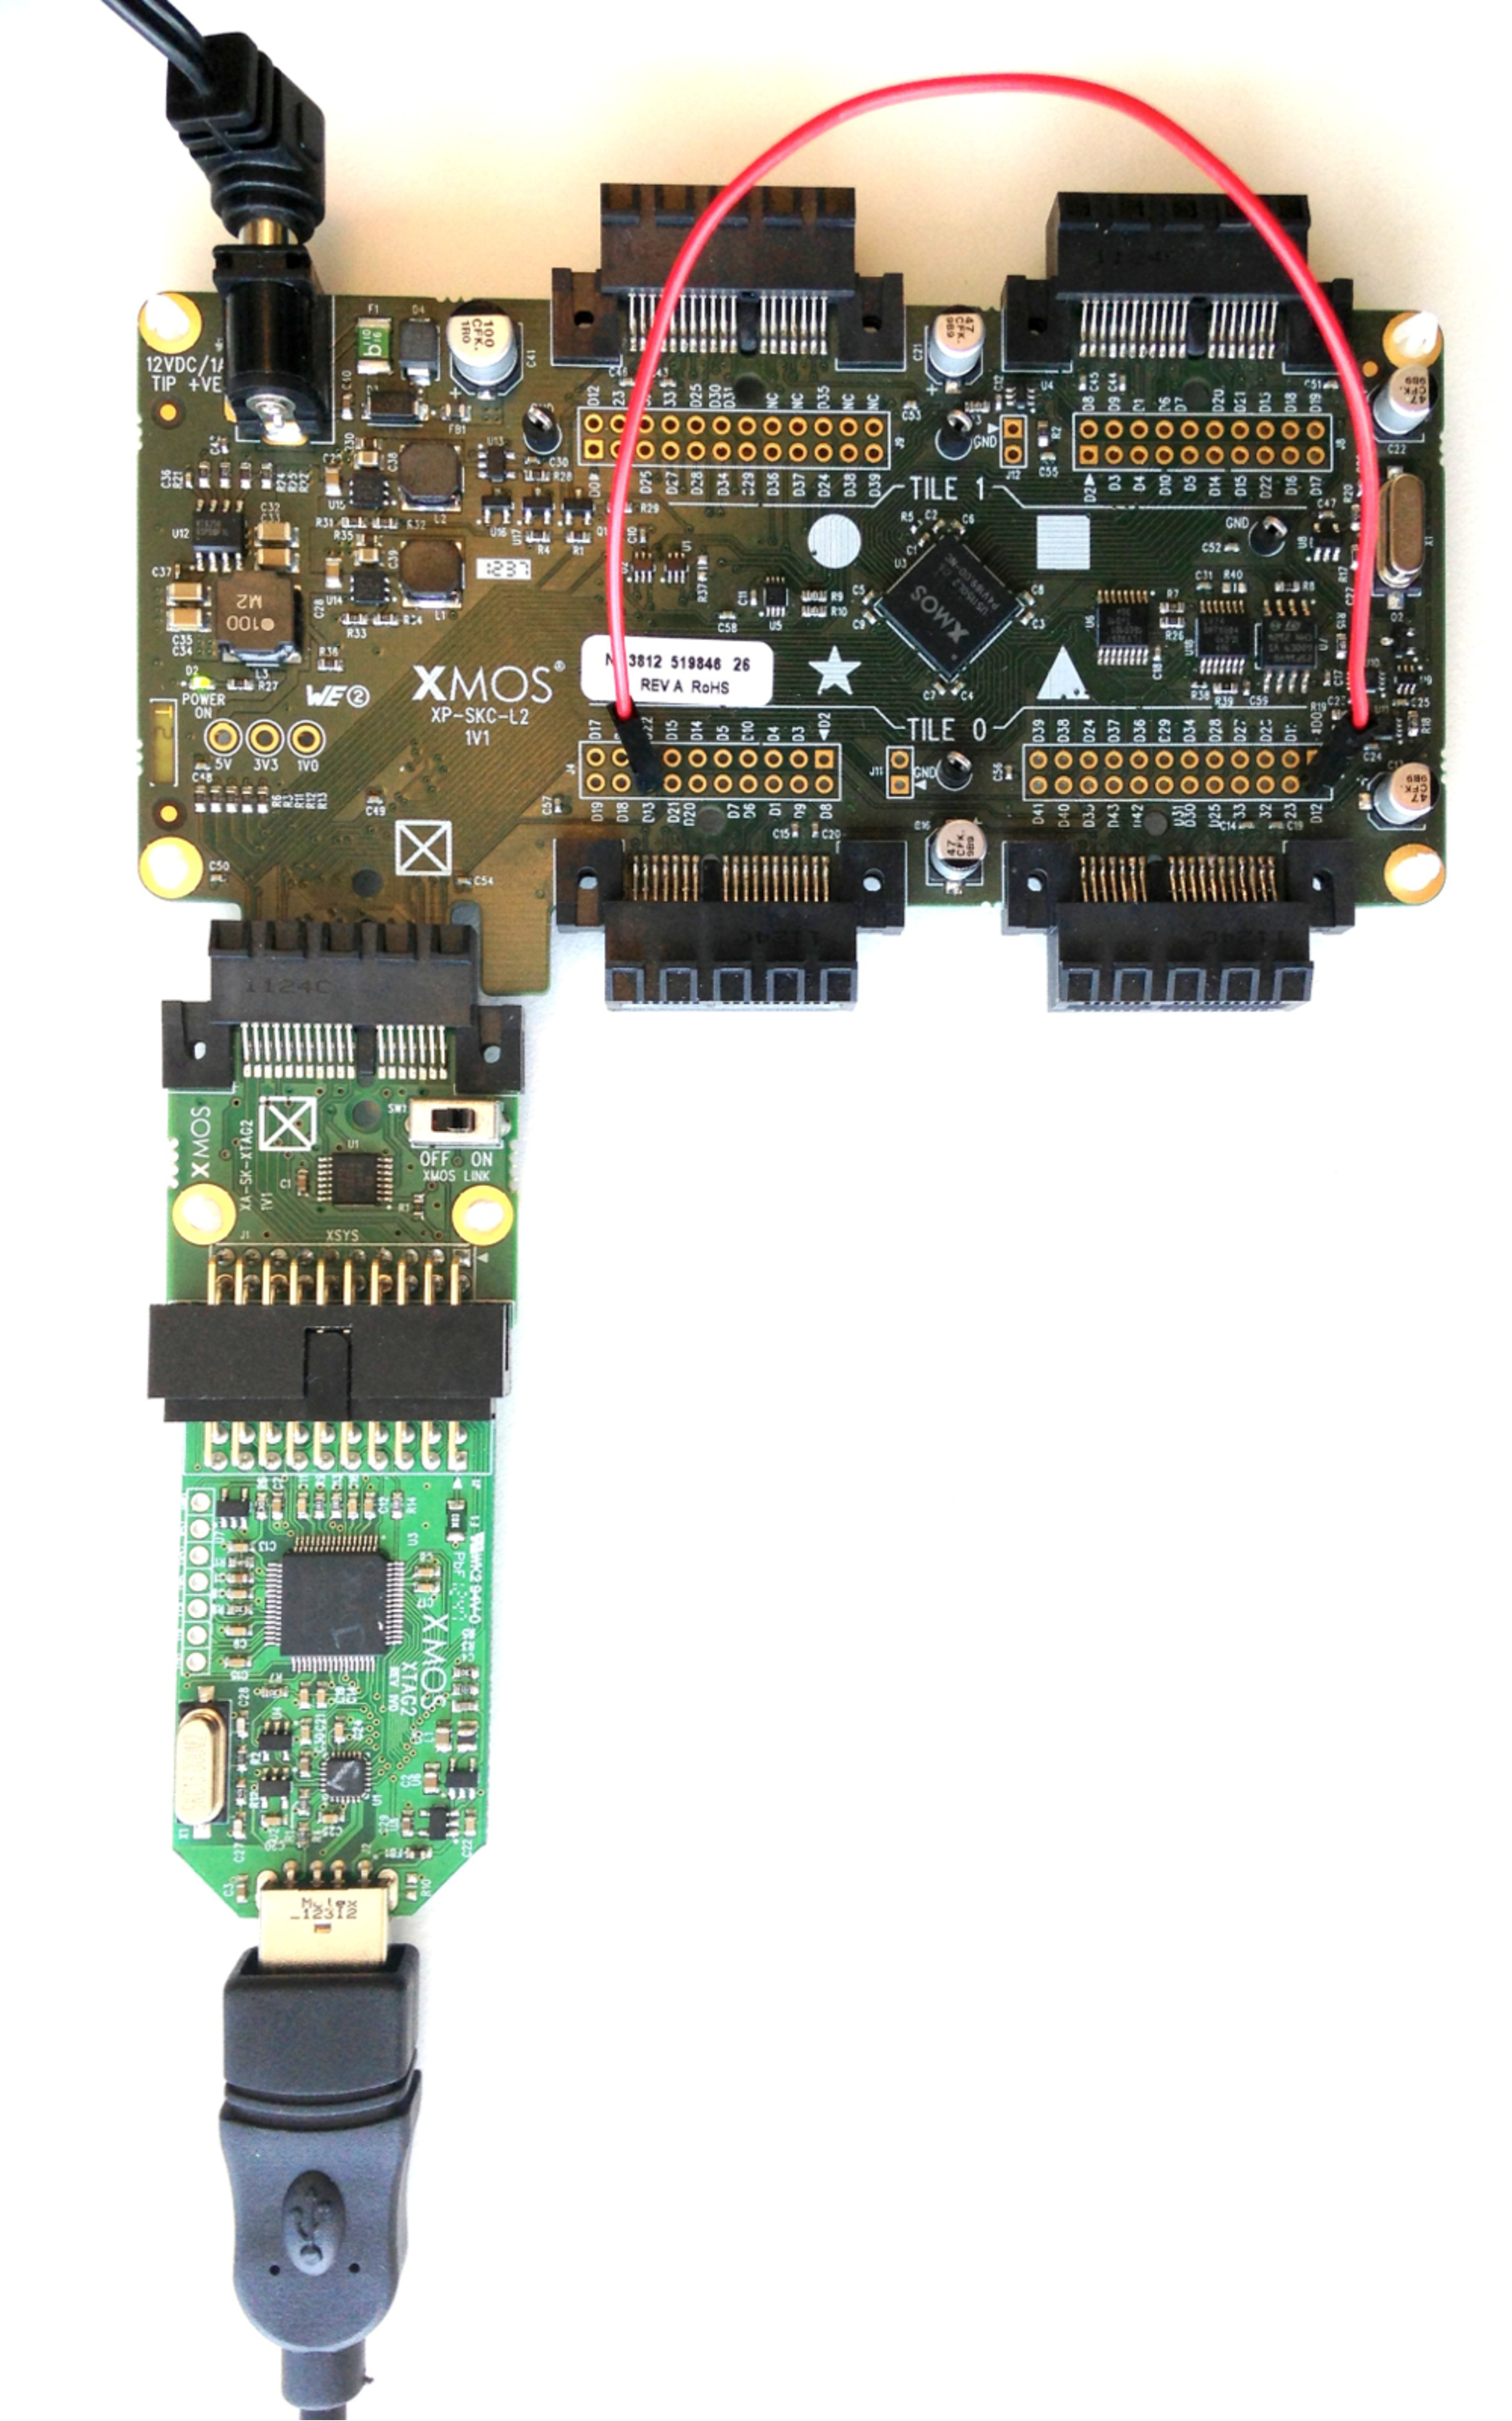
\includegraphics[width=75mm]{hardware_setup.pdf}
\end{sidecaption}\end{figure} \DocumentFooterFix



% NON-FULLWIDTH SECTION
\section{Import and Build the Application}
\label{quickstart:import-and-build-the-application}\begin{enumerate}
\item   Open xTIMEcomposer and check that it is operating in online mode. Open the edit perspective (Window-\textgreater{}Open Perspective-\textgreater{}XMOS Edit).

\item   Locate the \verb`'Simple/Fast Uart Loopback Example'` item in the xSOFTip pane on the bottom left of the window and drag it into the Project Explorer window in the xTIMEcomposer. This will also cause the modules on which this application depends (in this case, module\_uart\_rx \& module\_uart\_tx) to be imported as well.

\item   Click on the app\_uart\_fast item in the Project Explorer pane then click on the build icon (hammer) in xTIMEcomposer. Check the console window to verify that the application has built successfully.

\end{enumerate}



For help using xTIMEcomposer, try the xTIMEcomposer tutorial, which you can find by selecting Help-\textgreater{}Tutorials from the xTIMEcomposer menu.


Note that the Developer Column in the xTIMEcomposer, on the right hand side of your screen, provides information on the xSOFTip components you are using. Select the app\_uart\_fast component in the Project Explorer, and you will see its description together with API documentation. Having done this, click the \emph{back} icon until you return to this quickstart guide within the Developer Column.



% NON-FULLWIDTH SECTION
\section{Run the Application}
\label{quickstart:run-the-application}

Now that the application has been compiled, the next step is to run it on the Slicekit Core Board using the tools to load the application over JTAG (via the XTAG2 and XTAG Adapter card) into the xCORE multicore microcontroller.
\begin{enumerate}
\item   Select the file \verb`main.xc` in the \verb`app_uart_fast` project from the Project Explorer. This resides in the /src directory.

\item   Click on the \verb`Run` icon (the white arrow in the green circle).

\item   At the \verb`Select Device` dialog select \verb`XMOS XTAG-2 connect to L1[0..1]` and click \verb`OK`. If you only see \verb`Simulator` as the available target then please check to ensure the XTAG-2 debug adapter is properly connected to your PC.

\item   Proper operation of the application can be verified by observing the console window of xTIMEcomposer studio to see that the producer task has printed the success message \verb`Sent 32 characters in 23 microseconds.` and the consumer has verified the received array by printing \verb`Loopback test passed successfully.`. If the receiver does not print anything, or prints any statements like this \verb`Test failed. Value in array index..`, check to see that the loopback connection described in the hardware setup is correct.

\end{enumerate}




% NON-FULLWIDTH SECTION
\section{Next Steps}
\label{quickstart:next-steps}

Things to try now that the demo is running.
\begin{enumerate}
\item   Reduce the baud rate. Try changing the line \verb`#define BIT_PERIOD 10` to \verb`#define BIT_PERIOD 868`. This will cause the bit period to be 8680ns, which set the baud rate to 115Kbps (115207bps to be precise). You will see the resulting slower execution time of tx. The output should show \verb`Sent 32 characters in 1988 microseconds.`

\item   Break the link. Remove the flying loopback lead from rx to tx and run the app again, to verify that the loopback test fails.

\item   Change the tile the application is running on. Change \verb`#define DEMO_TILE 0` to  \verb`#define DEMO_TILE 1`.

\end{enumerate}



You must also change the flying lead to connect XD12 and XD13 to the \verb`SQUARE` and \verb`CIRCLE` side (tile 1). Build and run the application again. It is now running on a different tile to before.




\finish
